%% abtex2-modelo-projeto-pesquisa.tex, v-1.9.6 laurocesar
%% Copyright 2012-2016 by abnTeX2 group at http://www.abntex.net.br/ 
%%
%% This work may be distributed and/or modified under the
%% conditions of the LaTeX Project Public License, either version 1.3
%% of this license or (at your option) any later version.
%% The latest version of this license is in
%%   http://www.latex-project.org/lppl.txt
%% and version 1.3 or later is part of all distributions of LaTeX
%% version 2005/12/01 or later.
%%
%% This work has the LPPL maintenance status `maintained'.
%% 
%% The Current Maintainer of this work is the abnTeX2 team, led
%% by Lauro César Araujo. Further information are available on 
%% http://www.abntex.net.br/
%%
%% This work consists of the files abntex2-modelo-projeto-pesquisa.tex
%% and abntex2-modelo-references.bib
%%

% ------------------------------------------------------------------------
% ------------------------------------------------------------------------
% abnTeX2: Modelo de Projeto de pesquisa em conformidade com 
% ABNT NBR 15287:2011 Informação e documentação - Projeto de pesquisa -
% Apresentação 
% ------------------------------------------------------------------------ 
% ------------------------------------------------------------------------

\documentclass[
	% -- opções da classe memoir --
	12pt,				% tamanho da fonte
	openright,			% capítulos começam em pág ímpar (insere página vazia caso preciso)
	twoside,			% para impressão em recto e verso. Oposto a oneside
	a4paper,			% tamanho do papel. 
	% -- opções da classe abntex2 --
	%chapter=TITLE,		% títulos de capítulos convertidos em letras maiúsculas
	%section=TITLE,		% títulos de seções convertidos em letras maiúsculas
	%subsection=TITLE,	% títulos de subseções convertidos em letras maiúsculas
	%subsubsection=TITLE,% títulos de subsubseções convertidos em letras maiúsculas
	% -- opções do pacote babel --
	english,			% idioma adicional para hifenização
	brazil,				% o último idioma é o principal do documento
	]{abntex2}

% ---
% Formatação de código-fonte
% ---
\usepackage{listingsutf8}

% Altera o nome padrão do rótulo usado no comando \autoref{}
\renewcommand{\lstlistingname}{Código}

% Altera o rótulo a ser usando no elemento pré-textual "Lista de código"
\renewcommand{\lstlistlistingname}{Lista de códigos}

% Configura a ``Lista de Códigos'' conforme as regras da ABNT (para abnTeX2)
\begingroup\makeatletter
\let\newcounter\@gobble\let\setcounter\@gobbletwo
  \globaldefs\@ne \let\c@loldepth\@ne
  \newlistof{listings}{lol}{\lstlistlistingname}
  \newlistentry{lstlisting}{lol}{0}
\endgroup

\renewcommand{\cftlstlistingaftersnum}{\hfill--\hfill}

\let\oldlstlistoflistings\lstlistoflistings
\renewcommand{\lstlistoflistings}{%
   \begingroup%
   \let\oldnumberline\numberline%
   \renewcommand{\numberline}{\lstlistingname\space\oldnumberline}%
   \oldlstlistoflistings%
   \endgroup}
   

\lstset{
language = R,
numbers=left,
tabsize=2,
basicstyle=\footnotesize,
literate=
  {á}{{\'a}}1 {é}{{\'e}}1 {í}{{\'i}}1 {ó}{{\'o}}1 {ú}{{\'u}}1
  {Á}{{\'A}}1 {É}{{\'E}}1 {Í}{{\'I}}1 {Ó}{{\'O}}1 {Ú}{{\'U}}1
  {à}{{\`a}}1 {è}{{\`e}}1 {ì}{{\`i}}1 {ò}{{\`o}}1 {ù}{{\`u}}1
  {À}{{\`A}}1 {È}{{\'E}}1 {Ì}{{\`I}}1 {Ò}{{\`O}}1 {Ù}{{\`U}}1
  {ä}{{\"a}}1 {ë}{{\"e}}1 {ï}{{\"i}}1 {ö}{{\"o}}1 {ü}{{\"u}}1
  {Ä}{{\"A}}1 {Ë}{{\"E}}1 {Ï}{{\"I}}1 {Ö}{{\"O}}1 {Ü}{{\"U}}1
  {â}{{\^a}}1 {ê}{{\^e}}1 {î}{{\^i}}1 {ô}{{\^o}}1 {û}{{\^u}}1
  {Â}{{\^A}}1 {Ê}{{\^E}}1 {Î}{{\^I}}1 {Ô}{{\^O}}1 {Û}{{\^U}}1
  {œ}{{\oe}}1 {Œ}{{\OE}}1 {æ}{{\ae}}1 {Æ}{{\AE}}1 {ß}{{\ss}}1
  {ű}{{\H{u}}}1 {Ű}{{\H{U}}}1 {ő}{{\H{o}}}1 {Ő}{{\H{O}}}1
  {ç}{{\c c}}1 {Ç}{{\c C}}1 {ø}{{\o}}1 {å}{{\r a}}1 {Å}{{\r A}}1
  {€}{{\euro}}1 {£}{{\pounds}}1
}

% ---
% PACOTES
% ---

% ---
% Pacotes fundamentais 
% ---
\usepackage{lmodern}			% Usa a fonte Latin Modern
\usepackage[T1]{fontenc}		% Selecao de codigos de fonte.
\usepackage[utf8]{inputenc}		% Codificacao do documento (conversão automática dos acentos)
\usepackage{indentfirst}		% Indenta o primeiro parágrafo de cada seção.
\usepackage{color}				% Controle das cores
\usepackage{graphicx}			% Inclusão de gráficos
\usepackage{microtype} 			% para melhorias de justificação
\usepackage{colortbl}
\usepackage{csvsimple}
\usepackage{longtable}
\usepackage{tikz}
\usepackage{amsmath}




% ---

% ---
% Pacotes adicionais, usados apenas no âmbito do Modelo Canônico do abnteX2
% ---
% ---

% ---
% Pacotes de citações
% ---
\usepackage[brazilian,hyperpageref]{backref}	 % Paginas com as citações na bibl
\usepackage[alf]{abntex2cite}	% Citações padrão ABNT

% --- 
% CONFIGURAÇÕES DE PACOTES
% --- 

% ---
% Configurações do pacote backref
% Usado sem a opção hyperpageref de backref
\renewcommand{\backrefpagesname}{Citado na(s) página(s):~}
% Texto padrão antes do número das páginas
\renewcommand{\backref}{}
% Define os textos da citação
\renewcommand*{\backrefalt}[4]{
	\ifcase #1 %
		Nenhuma citação no texto.%
	\or
		Citado na página #2.%
	\else
		Citado #1 vezes nas páginas #2.%
	\fi}%
% ---

% ---
% Informações de dados para CAPA e FOLHA DE ROSTO
% ---
\titulo{Adaptação do algoritmo \textit{Particle Swarm Optimization} (PSO) para identificação de \textit{clusters} espaciais \\ Relatório Parcial}
\autor{Augusto Cesar Ribeiro Nunes}
\local{Brasília, Brasil}
\data{Novembro de 2016}
\instituicao{%
  Universidade de Brasília
  \par
  Departamento de Estatística
  \par
  Graduação}
\tipotrabalho{Trabalho de Conclusão de Curso (Graduação)}
% O preambulo deve conter o tipo do trabalho, o objetivo, 
% o nome da instituição e a área de concentração 
\preambulo{Relatório Parcial do Trabalho de Conclusão de Curso a ser apresentado para obtenção do título de Bacharel em Estatística. \newline \newline Orientador: Prof. Dr. \textbf{André Luiz Fernandes Cançado}}
% ---

% ---
% Configurações de aparência do PDF final

% alterando o aspecto da cor azul
\definecolor{blue}{RGB}{41,5,195}

% informações do PDF
\makeatletter
\hypersetup{
     	%pagebackref=true,
		pdftitle={\@title}, 
		pdfauthor={\@author},
    	pdfsubject={\imprimirpreambulo},
	    pdfcreator={LaTeX with abnTeX2},
		pdfkeywords={tcc}{trabalho de conclusão de curso}{estatística espacial}{estatística computacional}{Universidade de Brasília}{projeto de pesquisa}, 
		colorlinks=true,       		% false: boxed links; true: colored links
    	linkcolor=blue,          	% color of internal links
    	citecolor=blue,        		% color of links to bibliography
    	filecolor=magenta,      		% color of file links
		urlcolor=blue,
		bookmarksdepth=4
}
\makeatother
% --- 

% --- 
% Espaçamentos entre linhas e parágrafos 
% --- 

% O tamanho do parágrafo é dado por:
\setlength{\parindent}{1.3cm}

% Controle do espaçamento entre um parágrafo e outro:
\setlength{\parskip}{0.2cm}  % tente também \onelineskip

% ---
% compila o indice
% ---
\makeindex
% ---

% ----
% Início do documento
% ----
\begin{document}
\def\xlist{4}
\def\ylist{4}

\newcommand{\fillrandomly}[4]{
    \pgfmathsetmacro\diameter{#3*2}
    \draw (0,0) rectangle (#1,#2);
    \foreach \i in {1,...,#4}{
        \pgfmathsetmacro\x{rnd*#1}
        \pgfmathsetmacro\y{rnd*#2}
        \xdef\collision{0}
        \foreach \element [count=\i] in \xlist{
            \pgfmathtruncatemacro\j{\i-1}
            \pgfmathsetmacro\checkdistance{ sqrt( ({\xlist}[\j]-(\x))^2 + ({\ylist}[\j]-(\y))^2 ) }
            \ifdim\checkdistance pt<\diameter pt
                \xdef\collision{1}
                \breakforeach
            \fi
        }
        \ifnum\collision=0
            \xdef\xlist{\xlist,\x}
            \xdef\ylist{\ylist,\y}
            \draw [red, thick] (\x,\y) circle [radius=#3];
        \fi 

    }
}
% Seleciona o idioma do documento (conforme pacotes do babel)
%\selectlanguage{english}
\selectlanguage{brazil}

% Retira espaço extra obsoleto entre as frases.
\frenchspacing 

% ----------------------------------------------------------
% ELEMENTOS PRÉ-TEXTUAIS
% ----------------------------------------------------------
% \pretextual

% ---
% Capa
% ---
\imprimircapa
% ---

% ---
% Folha de rosto
% ---
\imprimirfolhaderosto
% ---

% ---
% NOTA DA ABNT NBR 15287:2011, p. 4:
%  ``Se exigido pela entidade, apresentar os dados curriculares do autor em
%     folha ou página distinta após a folha de rosto.''
% ---

% ---
% inserir lista de ilustrações
% ---
%\pdfbookmark[0]{\listfigurename}{lof}
%\listoffigures*
\cleardoublepage
% ---

% ---
% inserir lista de tabelas
% ---
%\pdfbookmark[0]{\listtablename}{lot}
%\listoftables*
\cleardoublepage
% ---

% ---
% inserir lista de abreviaturas e siglas
% ---
%\begin{siglas}
 % \item[PSO] \textit{Particle Swarm Optimization}
  %\item[abnTeX] ABsurdas Normas para TeX
%\end{siglas}
% ---

% ---
% inserir lista de símbolos
% ---
%\begin{simbolos}
%  \item[$ \Gamma $] Letra grega Gama
%  \item[$ \Lambda $] Lambda
%  \item[$ \zeta $] Letra grega minúscula zeta
%  \item[$ \in $] Pertence
%\end{simbolos}
% ---

% ---
% inserir o sumario
% ---
%\pdfbookmark[0]{\contentsname}{toc}
%\tableofcontents*
\cleardoublepage
% ---


% ----------------------------------------------------------
% ELEMENTOS TEXTUAIS
% ----------------------------------------------------------
\textual

% ----------------------------------------------------------
% Introdução
% ----------------------------------------------------------
\chapter*[Introdução]{Introdução}
\addcontentsline{toc}{chapter}{Introdução}

Este relatório parcial retrata o estado atual do trabalho de conclusão de curso em questão. Segundo o \nameref{chap:crono} do trabalho, aprovado em proposta de projeto, ele compreende o que foi feito dentre os meses de agosto e outubro de 2016.

A Análise e Identificação de \textit{clusters} é um problema da Estatística Espacial onde a heurística utilizada está intimamente ligada à natureza do fenômeno - sua dimensionalidade, a presença de uma estrutura de correlações relevante etc.

Temos em mãos um problema onde há a utilização de dados pontuais: registros das coordenadas ($X_i, Y_i$) do evento i; dados de área: onde não dispomos da localização precisa do evento mas sim de uma referência da área onde o mesmo ocorreu; e de dados de superfície: o elemento do conjunto de dados é formado por uma tripla ($X_i, Y_i, Z_i$) correspondente à coordenada geográfica do evento e a uma medição $Z_i$ realizada. Usualmente, ao analisar dados pontuais e dados de área, nosso interesse é por questões relativas à distribuição geográfica do processo pontual, quando o interesse se volta para dados de superfície, o interesse é por processos inferenciais que descrevam um modelo de probabilidade para o processo em questão.

O problema de identificação de \textit{clusters} a que este trabalho se dedica consiste em, ao analisar um espaço geográfico bidimensional G, particionado em regiões e no qual há a ocorrência de um processo pontual não-estocástico e dicotômico, avaliar se o mesmo ocorre de maneira meramente aleatória ou se há algum padrão definidor de um conglomerado, ou seja, tratamos de um processo pontual utilizando dados de área ao invés de dados pontuais. O motivador é o Algoritmo do \textit{Scan} Circular de Kulldorff, brevemente descrito em \ref{chap:ksc}. Apresentada por \cite{kulldorff1997spatial}, esta heurística simples e versátil tornou-se ubíqua graças a sua eficiência e interpretabilidade. O objetivo final do trabalho será obter um novo procedimento para a sua janela de análise (\textit{scan window}), que não será mais circular mas sim irá considerar um critério de adjacência, baseada no algoritmo \textit{Particle Swarm Optimization} (PSO).

O Algoritmo PSO por sua vez é muito brevemente descrito em \ref{chap:pso}. Proposto por \cite{eberhart1995new}, provou-se ser uma heurística de otimização robusta e cujas aplicações perpassam várias áreas, como mostram \cite{shi2001particle}.

O Capítulo \nameref{chap:parciais} e suas respectivas seções contém descrições dos passos já concluídos e resultados obtidos atee então. Dada a natureza essencialmente computacional do trabalho, eles decorrem diretamente das implementações e do código fonte apresentado no Apêndice \ref{apen:fonte}, que são citados ao longo do texto à medida que se faz necessária a referência.

No Capítulo \nameref{chap:posterior} é apresentada uma previsão tentada dos estágios imediatamente posteriores, sob uma ótica de planejamento.

Os conjuntos de dados utilizados no trabalho encontram-se no Anexo \ref{anex:dados}.


\chapter{O \textit{Scan} Circular de Kulldorff}
\label{chap:ksc}

\section{Descrição}
\cite{kulldorff1997spatial} tinha como um de seus objetivos estender a metodologia de detecção de conglomerados em um processo pontual unidimensional sugerida por \cite{naus1965distribution} a um contexto bidimension`al. Abordagens anteriores com o mesmo intuito usando processos de Poisson não-homogêneos \cite{weinstock1981generalised} e extensões do modelo Binomial \cite{saperstein1972generalized} resultaram em modelos de flexibilidade e eficiência questionáveis. A proposta de Kulldorff é significativamente mais simples e versátil, e a única limitação da análise é que há um condicionamento perene ao número total de casos observados. Suas prescrições são poucas e simples:

\begin{itemize}
\item Conhece-se a população sob risco do evento no espaço geográfico G e a mesma mantém-se constante durante a análise\footnote{Kulldorff também considerou modelos estocásticos em extensões de seu trabalho original};
\item Conhece-se o número de casos do evento no espaço geográfico G.
\item Bem como as coordenadas geográficas de ocorrência de todos estes eventos.
\end{itemize}

Seja G um Espaço Geográfico bidimensional onde há a presença de um processo pontual espacial N, onde N(A) é o número de pontos no conjunto $A \in G$. Conforme a janela de análise se movimenta sobre o Espaço Geográfico G, ela define uma coleção (uma zona) de regiões $\mathcal{Z} \in G$. Considerando um modelo Bernoulli para o processo pontual, temos que indivíduos que apresentam certa característica de interesse são pontos, e a localização destes indivíduos representa o processo pontual. No modelo, há exatamente uma zona $Z \in G$ tal que cada indivíduo dentro dela tem probabilidade p de ser um ponto (i.e. de possuir a característica de interesse), enquanto a probabilidade de indivíduos fora da zona em questão é q. A Figura \ref{fig:ksc1} abaixo ilustra o modelo neste estágio.

\begin{figure}
\centering
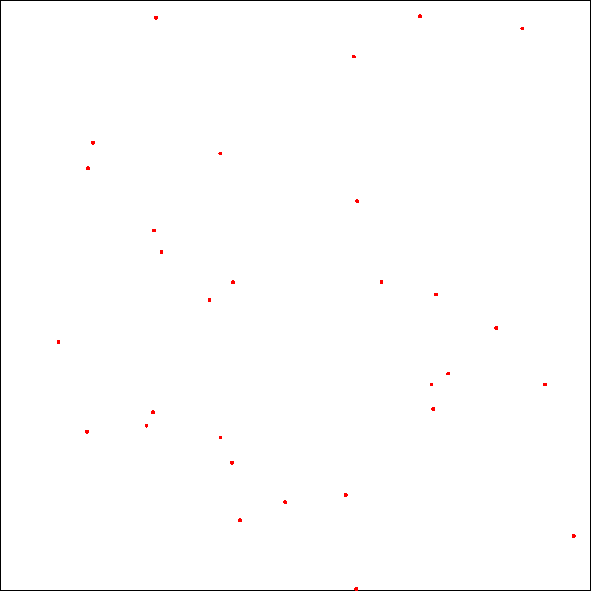
\includegraphics{tikz2_tec-figure0}
\caption{Modelo inicial do \textit{Scan} Circular de Kulldorff em um espaço geográfico com 30 casos (pontos vermelhos)} \label{fig:ksc1}
\end{figure}

A escolha do formato dos subconjuntos $A \in G$ varia de acordo com o contexto: bairros, ruas, distritos, quadrantes etc. Para facilitar a ilustração aqui utilizada, consideramos divisões em quadrados regulares, como na Figura \ref{fig:ksc2}. 

\begin{figure}
\centering
\begin{tikzpicture}
\node[anchor=south west,inner sep=0] at (0,0) {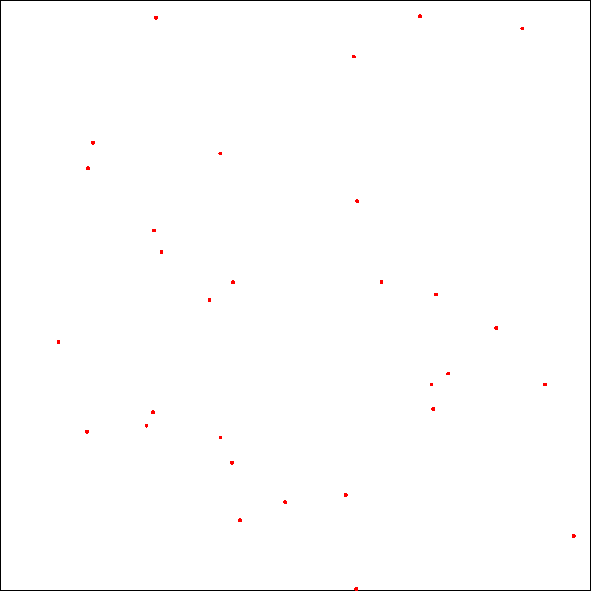
\includegraphics{tikz2_tec-figure0}};
\draw[help lines,xstep=2,ystep=2] (0,0) grid (10,10);
\end{tikzpicture}
\caption{Modelo do \textit{Scan} Circular de Kulldorff em um espaço geográfico com 30 casos e dividido em 25 regiões regulares. Cada uma dessas regiões é numerada.} \label{fig:ksc2}
\end{figure}

O passo a seguir pode ser considerado uma abstração útil: podemos definir um centroide\footnote{Aqui a definição de \textit{centroide} é \textit{ad hoc}: não corresponde necessariamente ao centro geométrico da região} onde estão \textit{condensados} todos os dados da região. A definição deste centroide pode partir de critérios práticos ou meramente geométricos: o caso inicial na região, uma unidade de saúde de referência, a prefeitura de cada cidade, uma instituição financeira etc. Essa medida mitiga o problema combinatório para a avaliação de conglomerados que surge quando n se torna suficientemente grande, mas ainda assim há prejuízo à eficiência do método quando a escolha das regiões e de seus centroides não é realizada de maneira cuidadosa. Em particular, o conjunto de dados utilizado no trabalho é artificial, e os centroides foram definidos com a introdução de um ruído aleatório às suas coordenadas x e y. Uma ilustração deste procedimento é feita na Figura \ref{fig:ksc3}


\begin{figure}
\centering
\begin{tikzpicture}
	\node[anchor=south west,inner sep=0] at (0,0) {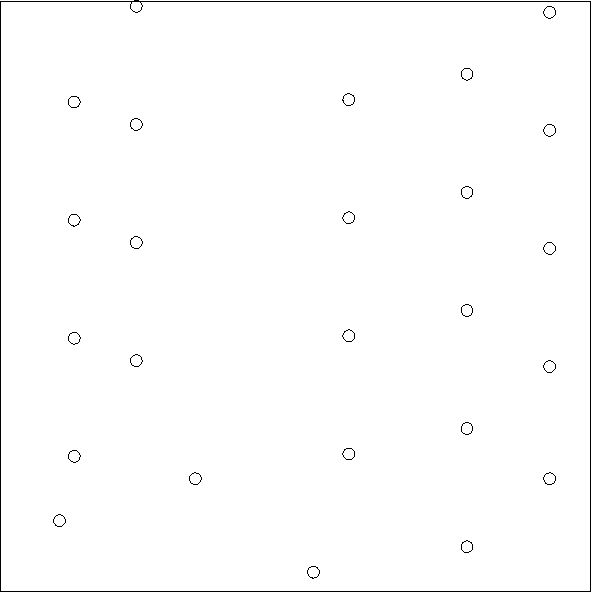
\includegraphics{tikz2_tec-figure1}};
	\draw[help lines,xstep=2,ystep=2] (0,0) grid (10,10);
	
\end{tikzpicture}
\caption{Modelo do \textit{Scan} Circular de Kulldorff obtido considerando os \textit{centroides} (circulos pretos) das regiões definidas anteriormente. Cada um dos 25 \textit{centroides} concentra todos os casos e a população da respectiva região} \label{fig:ksc3}
\end{figure}


O procedimento de identificação dos \textit{clusters} utiliza o Modelo Bernoulli e a razão de verossimilhança é obtida a partir das seguintes hipóteses:

\begin{align}
   H_0 & : p = q,   \qquad \text{para todo $\mathcal{Z} \in G$}
   \\
   H_1 & : p > q, \qquad \text{para algum $\mathcal{Z} \in G$}.
\end{align}

\begin{equation}
L(Z,p,q) = p^{n_Z}(1-p)^{\mu(Z) - n_Z}q^{n_G - n_Z}(1-q)^{(\mu(G) - \mu(Z)) - (n_G - n_Z)}
\label{eq:LLR}
\end{equation}

Onde $n_Z$ e $n_G$ são o número de caso observados na zona Z e em todo o espaço geográfico G, respectivamente; e $\mu(Z)$ e $\mu(G)$ são os casos esperados na zona Z e no espaço geográfico G, respectivamente. 

A próxima etapa, crucial, é a janela de análise do algoritmo propriamente dita:

\begin{enumerate}
\item Inicializar uma região\footnote{Poderia-se falar em \textit{centroide} e \textit{região} como sinônimos, a escolha pelo segundo termo é em nome da clareza.} qualquer;
\item Obter \ref{eq:LLR} para a região caso $n_Z > n_G$;
\item \textbf{Compor uma zona com a região inicial e a região cujo centroide seja o mais próximo do centroide inicial;}
\item Obter \ref{eq:LLR} para a região caso $n_Z > n_G$;
\item Repetir a composição em 3. e o cálculo de \ref{eq:LLR};
\item Parar quando o tamanho populacional da zona for maior que a metade do tamanho populacional total.
\end{enumerate} 

O Passo 3. é problemático: o critério de distância considera uma definição arbitrária - o centroide da região - e a janela de análise claramente cresce de maneira, como um \textbf{círculo} segundo o próprio nome do algoritmo sugere, o que afeta gravemente o poder do algoritmo na detecção de \textit{clusters} de formatos irregulares. Em \cite{kulldorff2006elliptic} o algoritmo da janela de análise foi estendido para considerar também formatos elípticos para o conglomerado. Ainda assim, a falta de flexibilidade do algoritmo, seja ele em formato circular ou elíptico, motiva fortemente a heurística considerada neste trabalho, descrita no capítulo a seguir.

Finalmente, a decisão para o teste das hipóteses 1.1 e 1.2 baseia-se em Simulação de Monte Carlo, procedimento descrito em \ref{chap:simmc}.



\chapter{O Algoritmo \textit{Particle Swarm Optimization} (PSO)}

O Algoritmo PSO tem como objetivo a otimização iterativa de funções não-lineares, e traz inspiração de comportamentos sociais biológicos como a revoada de aves e cardumes de peixes. 

Técnicas de \textit{Swarming}, termo que pode ser traduzido como \textit{enxameamento} e que foi sugerido inicialmente por \cite{beni1993swarm}, são amplamente utilizadas em contextos de Inteligência Artificial: a partir de um número considerável de agentes que interagem de maneira local e global, estes procedimentos buscam descrições de Estados Ótimos para os modelos. Estes \textit{Estados Ótimos} geralmente são os máximos globais de funções objetivo não-lineares.

O uso neste trabalho de um algoritmo \textit{baseado} no PSO se resumirá a encontrar uma maneira, ainda indefinida, para que a partir de uma série de zonas candidatas avalie-se interseções entre estas zonas e obtenha-se, assim, uma nova zona composta cuja forma não seja necessariamente regular, ao contrário do imposto pelo \textit{Scan} Circular de Kulldorff original. As prescrições e suposições do Modelo Bernoulli descritas no Capítulo \ref{chap:ksc} serão as mesmas: as únicas diferença serão a forma da janela de análise e a definição de um critério de decisão para identificar o \textit{cluster}.


% ----------------------------------------------------------
% Capitulo de textual  
% ----------------------------------------------------------
\chapter{Resultados Parciais}
\label{chap:parciais}
\section{\textit{Scan} Circular de Kulldorff}

Este algoritmo encontra-se implementado no \textit{software} SaTScan \cite{_satscan_????}, mantido pelo próprio Martin Kulldorff. Apesar de gratuito (i.e. distribuído sem ônus para o usuário), sua licença não é \textit{livre} na maioria das acepções utilizadas \cite{_free_????}, mais gravemente a não disponibilização de seu código-fonte. Isso impede, por exemplo, que utilizemos como base a implementação do SaTScan, feita em Java, para o R, o \textit{software} escolhido para implementação neste trabalho. Uma pesquisa no serviço \textit{crantastic} \cite{_its_????}, que disponibiliza uma ferramenta de busca nos pacotes disponíveis livremente para utilização no R, não retornou resultados para palavras-chave como "kulldorff circular scan", "circular scan" e similares. Uma pesquisa similar no \textit{github} também não retornou dentre os resultados implementações utilizáveis do \textit{Scan} Circular de Kulldorff.

Não obstante estas limitações, uma implementação \textit{inédita} do algoritmo serviu para facilitar grandemente a compreensão do mesmo, e de sua limitação que levou à proposição da nova heurística que serve como Objetivo deste trabalho. Ainda que o método sugerido por Kulldorff seja facilmente explicável em algumas palavras, colocá-lo em prática a partir do zero possibilitou uma familiarização importante.

O código-fonte em \ref{anex:scan-circular} é, apesar de correto, problemático em termos de eficiência do código. Uma análise de perfil (\textit{profiling}) do código utilizando a ferramenta \texttt{Rprofvis} do R, disponível em \cite{_rpubs_????}, mostra o culpado: o incremento iterativo do \textit{data frame} \texttt{resultado}. Este tipo de erro é comum, sendo inclusive citado no texto "The R Inferno" \cite{burns2012r}, do consultor Patrick Burns. Na verdade, sua solução é, em teoria, simples: via de regra a alocação de uma estrutura de dados qualquer previamente considerando seu tamanho final ou máximo sempre será mais eficiente que sua alocação iterativa. Como o objetivo maior do trabalho não envolve uma implementação eficiente do \textit{Scan} Circular, não há inicialmente a preocupação em mitigar o efeito da técnica flagrantemente ineficaz de alocação de dados. 

Ainda sobre o código-fonte, sua leitura deve ser razoavelmente intuitiva mas ele essencialmente especifica uma função que realiza duas coisas, a saber: 

\begin{itemize}
\item Obtém a matriz de distâncias dos centroides das regiões utilizando distância euclidiana.
\item Calcula o logaritmo da razão de verossimilhança para cada uma das zonas candidatas.
\end{itemize}

Estas zonas são nada mais do que composições de regiões, e como o nome sugere e deve ficar claro à leitura do código-fonte a heurística de composição destas zonas é a distância a partir de um centroide inicial até os centroides das outras regiões no espaço.

\newpage
\section{Simulação de Monte-Carlo}
\label{sec:simmc}
Na etapa seguinte, foi feita a verificação de significância do \textit{cluster} mais verossímil, i.e. cujo logaritmo da razão de verossimilhança seja maior. A hipótese nula a ser testada é de que a probabilidade de ocorrência do evento \textit{dentro} da zona candidata que apresenta o maior valor da estatística em questão é igual à probabilidade de ocorrência do evento fora desta zona em particular.

Para tanto, podemos gerar um número \textit{considerável} de realizações de uma distribuição Multinomial sob hipótese nula, ou seja, cujas componentes do seu vetor de probabilidade são proporcionais ao produto entre a razão do total de casos sobre a população total e a população na região. Em notação usual, foram geradas realização de uma variável aleatória $X \sim (\sum_i P_i, \mu_0 P_1, \mu_0 P_2, \dots, \mu_n P_n)$, onde $\mu_0$ é a média geral sob a hipótese nula, e $P_i, i=1,\dots, n$ é a população na região i.

De acordo com o conjunto de dados aqui utilizado, disponibilizado pelo orientador, chegou-se à conclusão de que a zona formada pelas regiões 130, 131, 143, 144, 145, 157, 158 têm probabilidade de ocorrência do evento significativamente superior à observada nas outras zonas. 

O baixo número de realizações da simulação dá-se em parte por conta da falta de eficiência do \textit{Scan} Circular retratada na seção anterior. Ainda assim, o resultado observado no trabalho condiz com o resultado obtido previamente pelo orientador.



\chapter{Próximos Passos}
\label{chap:posterior}

Há a tentativa de implementação de uma heurística para composição das zonas que não leve em consideração a distância entre os centroides, mas sim quais apresentam a propriedade de adjacência entre si. Este algoritmo estaria descrito, grosso modo, nos seguintes termos.

\begin{enumerate}
\item Inicializa-se uma região i qualquer.
\item A partir de i, e tendo acesso a quais regiões são adjacentes a i, obter a zona onde o logaritmo da razão de verossimilhança é maior quando há a composição da região i com suas adjacentes.
\item A partir da zona composta pelas duas regiões, i e aquela que mais aumenta a razão de verossimilhança, compor um vetor de vizinhanças para a zona a partir das regiões que a compõem.
\item Pare quando o tamanho populacional da zona for maior que metade da população total.
\end{enumerate}

Eventualmente, o procedimento descrito acima encontrará um certo número de \textit{zonas candidatas}. A partir destas zonas candidatas, a intenção é trabalhar com zonas candidatas que apresentem interseção entre si e compô-las de forma que possam apresentar formatos não-regulares.

\chapter{Cronograma}
\label{chap:crono}

As atividades a serem desenvolvidas são as seguintes:

\begin{enumerate}
	\item \label{etapa1} Escolha do tema a ser abordado.
	\item \label{etapa2} Desenvolvimento da proposta de projeto.
	\item \label{etapa3} Entrega da proposta de projeto.
	\item \label{etapa4} Revisão de literatura.
	\item \label{etapa5} Elaboração da apresentação da proposta.
	\item \label{etapa6} Apresentação oral da proposta.
	\item \label{etapa7} Implementação
    \item \label{etapa8} Verificação dos Modelos
	\item \label{etapa9} Elaboração do relatório parcial.
	\item \label{etapa10} Entrega do relatório parcial ao Professor Orientador.
	\item \label{etapa11} Correção do relatório parcial.
	\item \label{etapa12} Entrega do relatório parcial para a banca.
	\item \label{etapa13} Desenvolvimento do modelo.
    \item \label{etapa14} Elaboração do relatório final.
	\item \label{etapa15} Entrega do relatório final ao Professor Orientador.
	\item \label{etapa16} Correção do do relatório final.
	\item \label{etapa17} Entrega do relatório final para a banca.
\end{enumerate}

\definecolor{midgray}{gray}{.5}
\def\tablename{Tabela }%
\begin{table}[!htbp]\scriptsize
\centering {\caption{Cronograma}
		\begin{tabular}{|c|c|c|c|c|c|c|c|c|c|c|c|c|}
		\hline
		&\multicolumn{5}{c|}{2016}&\multicolumn{7}{c|}{2017}\\
		\hline
		&Agosto&Setembro&Outubro&Novembro&Dezembro&Janeiro&Fevereiro&Março&Abril&Maio&Junho&Julho\\
		\hline
		\ref{etapa1}&\cellcolor{midgray}&&&&&&&&&&&\\
		\hline
		\ref{etapa2}&&\cellcolor{midgray}&&&&&&&&&&\\
		\hline	
		\ref{etapa3}&&\cellcolor{midgray}&&&&&&&&&&\\
		\hline			
		\ref{etapa4}&&\cellcolor{midgray}&\cellcolor{midgray}&&&&&&&&&\\
		\hline	
		\ref{etapa5}&&&\cellcolor{midgray}&&&&&&&&&\\
		\hline
		\ref{etapa6}&&&\cellcolor{midgray}&\cellcolor{midgray}&&&&&&&&\\
		\hline	
		\ref{etapa7}&\cellcolor{midgray}&\cellcolor{midgray}&\cellcolor{midgray}&\cellcolor{midgray}&\cellcolor{midgray}&&&&&&&\\
		\hline	
		\ref{etapa8}&&&\cellcolor{midgray}&&&\cellcolor{midgray}&&&&&&\\
		\hline	
		\ref{etapa9}&&&&&\cellcolor{midgray}&&&&&&&\\
		\hline	
		\ref{etapa10}&&&&&&\cellcolor{midgray}&&&&&&\\
		\hline	
		\ref{etapa11}&&&&&&\cellcolor{midgray}&\cellcolor{midgray}&\cellcolor{midgray}&&&&\\
		\hline	
		\ref{etapa12}&&&&&&&&\cellcolor{midgray}&\cellcolor{midgray}&&&\\
		\hline	
		\ref{etapa13}&&&&&&&&\cellcolor{midgray}&\cellcolor{midgray}&\cellcolor{midgray}&&\\
        \hline
        \ref{etapa14}&&&&&&&&&\cellcolor{midgray}&\cellcolor{midgray}&\cellcolor{midgray}&\\
        \hline
        \ref{etapa15}&&&&&&&&&&\cellcolor{midgray}&&\\
        \hline
        \ref{etapa16}&&&&&&&&&&\cellcolor{midgray}&\cellcolor{midgray}&\\
        \hline	
        \ref{etapa17}&&&&&&&&&&&&\cellcolor{midgray}\\
        \hline
		\end{tabular}}
\end{table}


% ----------------------------------------------------------
% ELEMENTOS PÓS-TEXTUAIS
% ----------------------------------------------------------
\postextual

% ----------------------------------------------------------
% Referências bibliográficas
% ----------------------------------------------------------
\bibliography{proj}

% ----------------------------------------------------------
% Glossário
% ----------------------------------------------------------
%
% Consulte o manual da classe abntex2 para orientações sobre o glossário.
%
%\glossary

% ----------------------------------------------------------
% Apêndices
% ----------------------------------------------------------

% ---
% Inicia os anexos
% ---
\begin{apendicesenv}

% Imprime uma página indicando o início dos anexos
\partanexos


% ---
\chapter{Códigos-fonte}
\label{apen:fonte}

Os códigos-fonte aqui disponibilizados encontram-se  hospedados no repositório \url{https://github.com/august-o/tcc}.


\section{\textit{Scan} Circular de Kulldorff}
\label{anex:scan-circular}
% ---
\lstinputlisting{llr_ksc.R}


% ---
\section{Simulação de Monte-Carlo}
\lstinputlisting{sim.ksc.R}

\end{apendicesenv}

\begin{anexosenv}



\chapter{Conjuntos de Dados}
\label{anex:dados}

Os conjuntos de dados utilizados neste trabalho encontram-se hospedados no repositório \url{https://github.com/august-o/tcc/tree/master/dados_hex}. 

\section{dados.csv}

Arquivo tabulado que descreve o número de casos observados e a população de 203 regiões, bem como as coordenadas de seus \textit{centroides}.

\section{hex.adj}

Matriz de adjacências para as 203 regiões. A componente (i,j) nesta matriz é igual a 1 se as regiões i e j são adjacentes entre si e 0 caso contrário.
\end{anexosenv}

\phantompart

\printindex


\end{document}
